% Reporte técnico de percepcion_nav (FR-055). Compilar dos veces:
%   cd percepcion_nav/docs/reporte && pdflatex reporte_tecnico.tex && pdflatex reporte_tecnico.tex
\documentclass[9pt,letterpaper]{extarticle}
\usepackage[T1]{fontenc}
\usepackage{lmodern}
\usepackage{babel}
\babelprovide[import, main]{spanish}
\usepackage[margin=1.35cm, top=1.2cm, bottom=1.3cm]{geometry}
\usepackage{graphicx}
\usepackage{booktabs}
\usepackage{tabularx}
\usepackage{multicol}
\usepackage{amsmath}
\usepackage{amssymb}
\usepackage[font=footnotesize, labelfont=bf, skip=2pt]{caption}
\usepackage{subcaption}
\usepackage{enumitem}
\usepackage{xcolor}
\usepackage{float}
\usepackage{microtype}
\usepackage[hidelinks]{hyperref}

\graphicspath{{figuras/}}
\setlist{nosep, leftmargin=1.1em}
\setlength{\parskip}{0.25em}
\setlength{\parindent}{0pt}
\setlength{\columnsep}{0.55cm}
\setlength{\abovedisplayskip}{3pt}
\setlength{\belowdisplayskip}{3pt}
\newcommand{\code}[1]{\texttt{\small #1}}
\newcommand{\pendiente}[1]{\textcolor{red}{[pendiente: #1]}}
\newcommand{\ok}{\textcolor{green!50!black}{\checkmark}}
\renewcommand{\arraystretch}{1.05}
\pagestyle{plain}

\begin{document}

\begin{center}
  {\Large\bfseries Paquete ROS 2 de percepción para navegación}\\[2pt]
  {\small José Ángel Balbuena Palma \;·\; MPIAF-12 Visión Inteligente, Tema 5, actividad integradora \;·\;
  Maestría en IA, TecNM Atlixco \;·\; 6 de octubre de 2026}
\end{center}

\section*{1. Arquitectura}

El paquete \code{percepcion\_nav} (ROS~2 Jazzy, \code{ament\_python}) reparte el pipeline en cinco
nodos desacoplados y una herramienta de prueba. Se comunican solo por tópicos estándar, tf2 y la
acción \code{NavigateToPose}. Hay tres lanzamientos: \textbf{pipeline 2D} (video real),
\textbf{\code{dry\_run}} (cadena completa con profundidad sintética y tf estático, sin servidor de
navegación) y \textbf{simulación} (Gazebo Harmonic, TurtleBot~4 de Nav2, silla modelada en FreeCAD y
Nav2 real). Entre un modo y otro solo cambian remapeos y parámetros, nunca el código.

\begin{figure}[H]
  \centering
  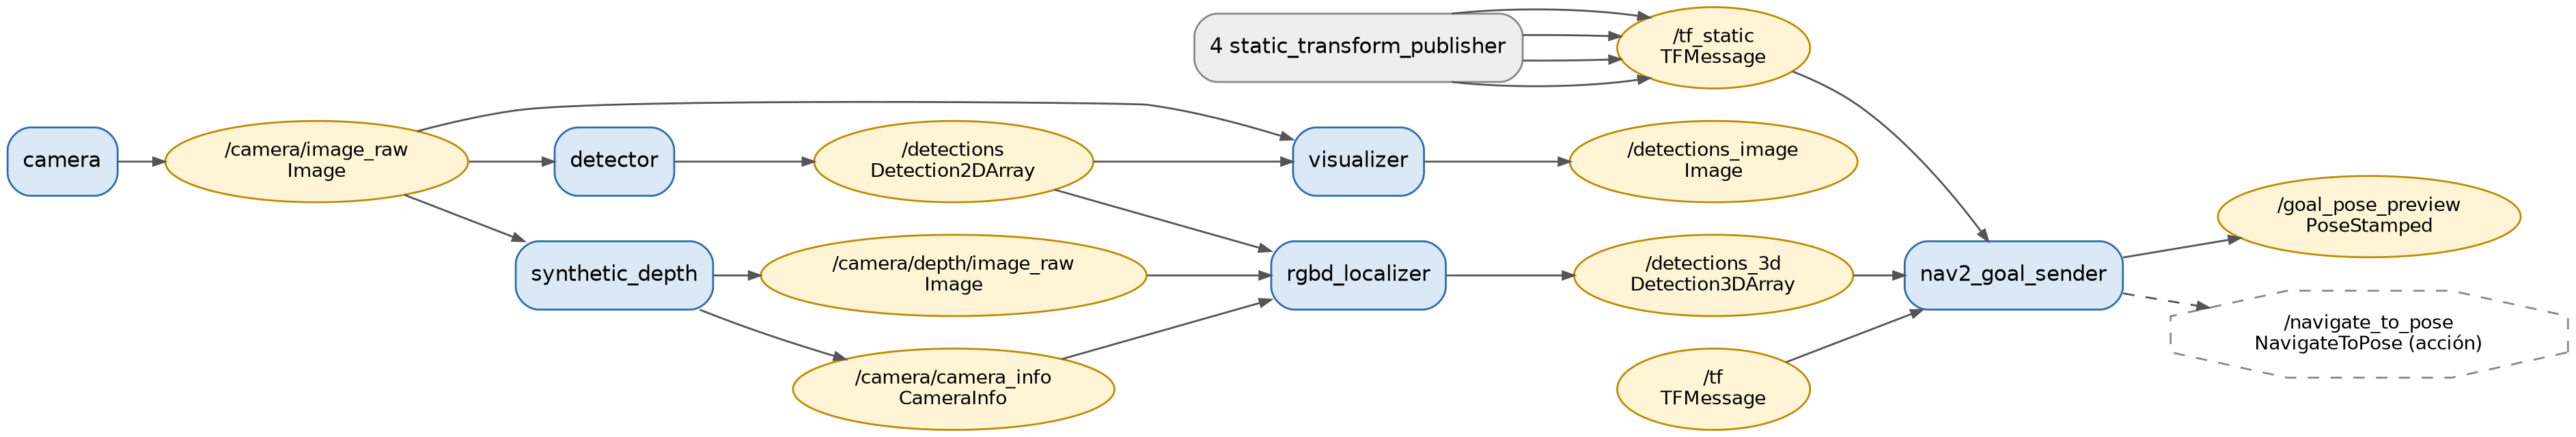
\includegraphics[width=\linewidth]{grafo_dry_run.png}
  \caption{Grafo de nodos (azul) y tópicos (amarillo) del sistema en \code{dry\_run}, obtenido por
  introspección del grafo de ROS en ejecución. La acción (línea punteada) solo se usa con
  \code{dry\_run:=false}. En simulación, \code{camera} y \code{synthetic\_depth} se sustituyen por
  la cámara RGB-D simulada mediante remapeos.}
  \label{fig:grafo}
\end{figure}

\begin{multicols}{2}
\section*{2. Decisiones de diseño}
\begin{itemize}
  \item \textbf{Solo mensajes estándar:} \code{Image}, \code{CameraInfo},
        \code{Detection2DArray}, \code{Detection3DArray}, \code{PoseStamped} y
        \code{NavigateToPose}. Cada \code{Detection2D} lleva bbox en píxeles, \code{class\_id},
        \code{score} y el \code{header} de su imagen.
  \item \textbf{QoS:} publicadores \emph{reliable} y suscriptores de imagen \emph{best effort}. El
        detector usa cola de 1 y procesa siempre el cuadro más reciente.
  \item \textbf{Estampas:} el detector copia el \code{header} de la imagen. La visualización
        empareja por estampa exacta y el localizador por estampa aproximada ($\le 20$~ms), con
        colas que cubren la latencia de la inferencia.
  \item \textbf{tf2:} consultas en la estampa de la detección, con tiempo límite. Un ejecutor
        multihilo y un listener reentrante permiten esperar sin bloquear \code{/tf}.
  \item \textbf{Robustez:} ningún error recuperable termina un nodo (fuente ausente,
        conversión, profundidad inválida, tf, servidor ausente). Los avisos tienen límite de
        frecuencia. Si faltan los pesos del modelo, el nodo falla al arrancar.
  \item \textbf{Entorno:} \code{.venv} con \code{--system-site-packages} y \code{numpy<2} (por
        \code{cv\_bridge}). Se compila sin \code{--symlink-install}, porque ese modo ignora el
        intérprete del \code{.venv} (verificado).
\end{itemize}

\section*{3. Componente RGB-D}
Para cada detección se toma una ventana central del bbox (30\,\% de su ancho y alto) y se estima
$Z$ como la \textbf{mediana} de los píxeles finitos y positivos. \code{16UC1} se convierte de mm a
m. El centro del bbox se deproyecta con el modelo pinhole:
\[
  X = \frac{(u-c_x)\,Z}{f_x},\qquad Y = \frac{(v-c_y)\,Z}{f_y}.
\]
La cámara solo ve la cara frontal del objeto. En simulación se activa \code{estimate\_center}, que
avanza sobre el rayo la mitad del ancho métrico $w Z/f_x$ (supuesto de huella cuadrada). Sin esa
corrección, la estimación quedaba a 0.25~m del centro de la silla; con ella, a 0.04~m.

\section*{4. Conexión con Nav2}
El punto se transforma a \code{map} y la pose del robot $r$ sale de \code{map}$\to$\code{base\_link},
ambos en la estampa de la detección. La meta queda a $d=1.0$~m del objeto $o$, mirándolo:
\[
  g = o - d\,\frac{o-r}{\lVert o-r\rVert},\qquad \psi=\operatorname{atan2}(o_y-g_y,\;o_x-g_x).
\]
No se envía meta si $\lVert o-r\rVert \le d+0.30$~m. Con una meta activa no se reenvía salvo que
el objetivo se mueva más de 0.5~m, y se descartan las detecciones anteriores al último resultado.
La espera del servidor está limitada y se registran la aceptación, el progreso y el resultado.
\end{multicols}

\vspace{-6pt}
\begin{figure}[H]
  \centering
  \begin{subfigure}[b]{0.60\linewidth}
    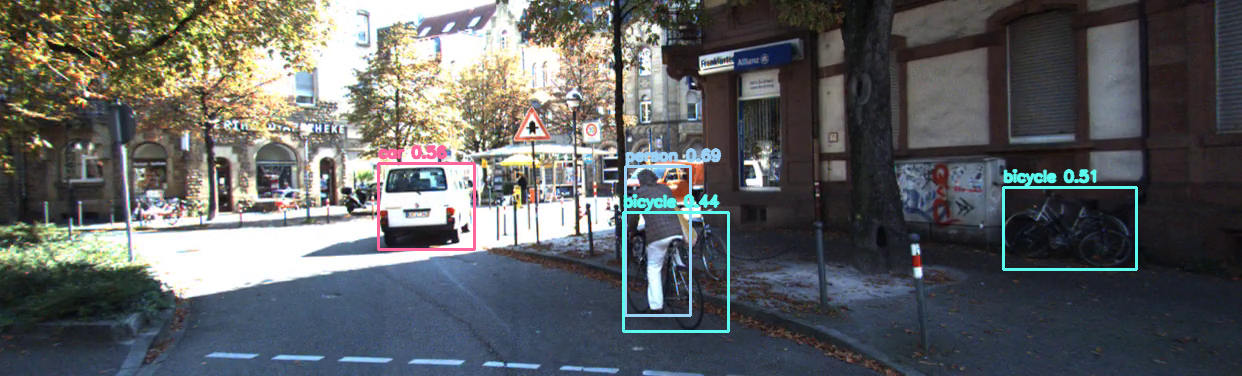
\includegraphics[width=\linewidth]{pipeline_2d.png}
    \caption{Pipeline 2D: \code{/detections\_image} (primera imagen anotada a los 5.8~s;
    5.3--8.9 detecciones/s en CPU). Video de prueba con cuadros del conjunto KITTI.}
  \end{subfigure}\hfill
  \begin{subfigure}[b]{0.37\linewidth}
    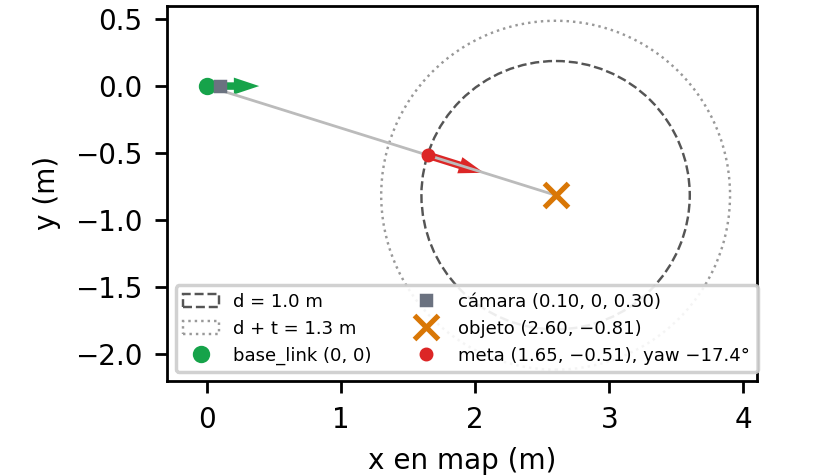
\includegraphics[width=\linewidth]{dry_run_geometria.png}
    \caption{\code{dry\_run}: objeto en \code{map} con profundidad sintética de 2.5~m; meta medida
    a 1.000~m del objeto, orientada hacia él.}
  \end{subfigure}
  \caption{Ejecución real del pipeline 2D y del cálculo de la meta sin robot.}
\end{figure}

\newpage
\section*{5. Simulación frente a posición real}
\vspace{-2pt}
\begin{figure}[H]
  \centering
  \begin{subfigure}[b]{0.64\linewidth}
    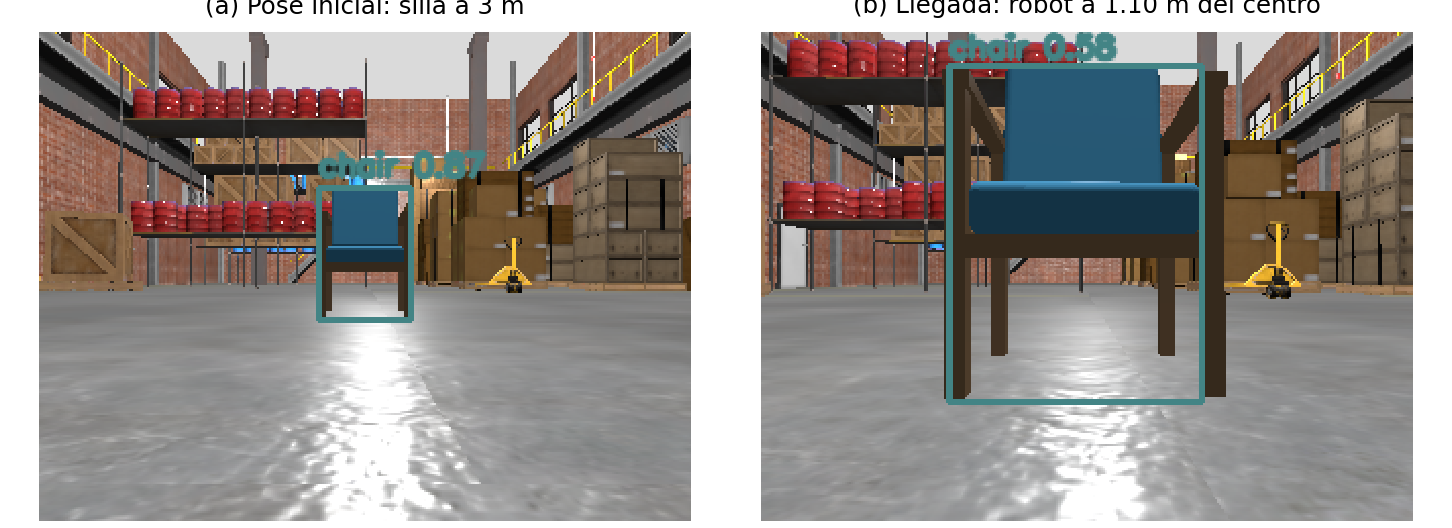
\includegraphics[width=\linewidth]{sim_camara.png}
    \caption{Cámara RGB-D simulada con las detecciones del pipeline.}
  \end{subfigure}\hfill
  \begin{subfigure}[b]{0.345\linewidth}
    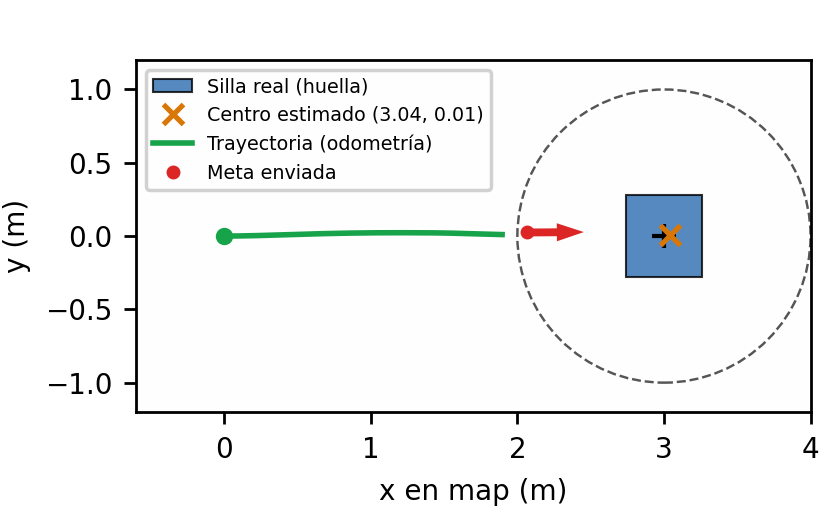
\includegraphics[width=\linewidth]{sim_trayectoria.png}
    \caption{Trayectoria sobre el mapa \code{depot}.}
  \end{subfigure}\\[2pt]
  \begin{subfigure}[b]{0.92\linewidth}
    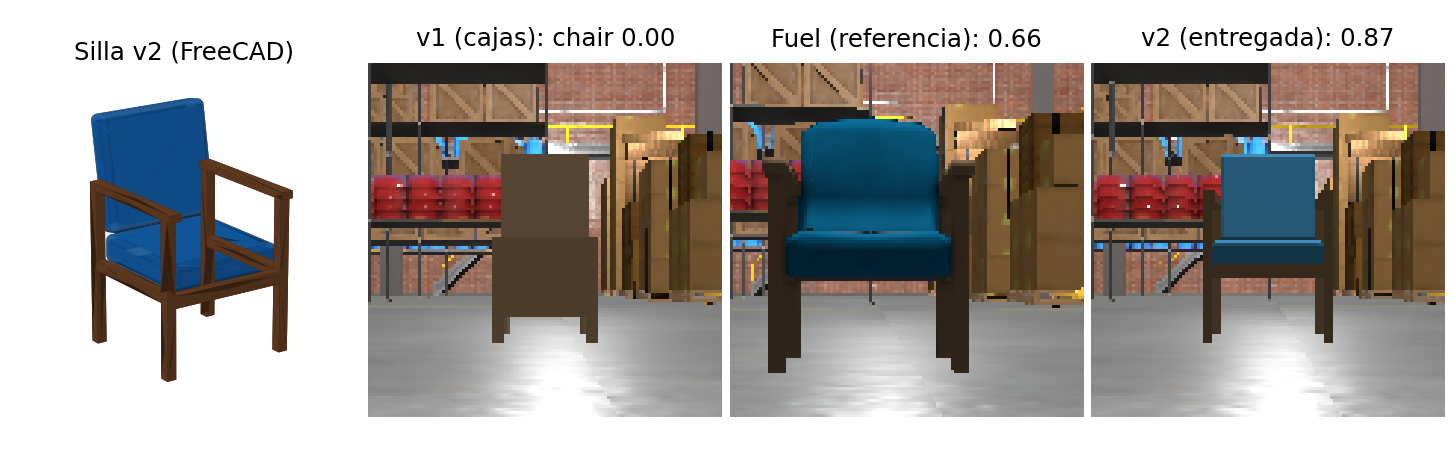
\includegraphics[width=\linewidth]{silla_iteraciones.png}
    \caption{Silla de FreeCAD y score de \code{chair} de YOLO11n desde la pose inicial: la v1
    (cajas) no se reconocía. La v2 (estructura y cojines) es la que se usa.}
  \end{subfigure}
  \caption{Simulación (Gazebo con render por software, factor de tiempo real 0.49). La silla está
  en \code{map}~(3.0,~0.0). La pose real del robot se toma de la odometría ideal de Gazebo.}
\end{figure}

\vspace{-6pt}
\begin{table}[H]
  \centering\footnotesize
  \caption{Cinco corridas independientes. Las distancias se miden al centro de la huella de la
  silla.}
  \begin{tabular}{@{}cccccc@{}}
    \toprule
    Corrida & Error de la estimación & Distancia final & Error de orientación & Resultado de la acción & Metas tras llegar \\
            & (SC-008, $\le 0.30$~m) & (SC-009, $1.0\pm0.30$~m) & (SC-009, $\le 15^\circ$) & & (FR-042) \\
    \midrule
    1 & 0.04~m \ok & 1.025~m \ok & $1.4^\circ$ \ok & \code{SUCCEEDED} & 0 \\
    2 & 0.04~m \ok & 1.088~m \ok & $1.3^\circ$ \ok & \code{SUCCEEDED} & 0 \\
    3 & 0.04~m \ok & 1.071~m \ok & $0.9^\circ$ \ok & \code{SUCCEEDED} & 0 \\
    4 & 0.04~m \ok & 1.097~m \ok & $2.2^\circ$ \ok & \code{SUCCEEDED} & 0 \\
    5 & 0.04~m \ok & 1.082~m \ok & $2.2^\circ$ \ok & \code{SUCCEEDED} & 0 \\
    \bottomrule
  \end{tabular}
\end{table}

\vspace{-8pt}
\section*{6. Validado frente a diseño}
\vspace{-2pt}
{\footnotesize
\begin{tabularx}{\linewidth}{@{}lXl@{}}
  \toprule
  Componente & Cómo se validó & Quedó sin probar \\
  \midrule
  Cámara & Ejecución real con video; fuente ausente con reintentos y recuperación en 1.9~s;
           fin de video con salida limpia & Webcam física (WSL2 no la expone) \\
  Detector & Ejecución real; \code{Detection2DArray} completo y con el \code{header} de la imagen;
             5 pruebas de construcción de mensajes & Rendimiento con GPU \\
  Visualización & Ejecución real (Fig.~2a) y en simulación (Fig.~3a) & --- \\
  RGB-D & 21 pruebas \code{pytest} sin ROS (error de deproyección $<1$~mm); \code{dry\_run}
          ($z=2.50$~m); simulación (error de 0.04~m) & Sensor físico: ruido y alineación real \\
  Nav2 & 9 pruebas sin ROS (1~cm, $<1^\circ$); \code{dry\_run}; Nav2 real en simulación, 5/5
         corridas \code{SUCCEEDED} & Robot físico \\
  \bottomrule
\end{tabularx}}

\section*{7. Autoevaluación (rúbrica, 0 a 4)}
\vspace{-2pt}
{\footnotesize
\begin{tabularx}{\linewidth}{@{}lcX@{}}
  \toprule
  Criterio & Nivel & Evidencia \\
  \midrule
  Nodo de cámara & 4 & \code{Image} con estampa y \code{frame\_id}; manejo de errores con
                       reintentos (§6); video de demostración \pendiente{minuto} \\
  Detector con \code{vision\_msgs} & 4 & \code{Detection2DArray} con bbox, clase y score (§2,
                       Fig.~2a); pruebas automáticas \\
  Verificación visual & 4 & Imagen anotada de extremo a extremo (Fig.~2a y 3a); grafo
                       (Fig.~1) \\
  Componente RGB-D & 4 & Implementado, justificado (§3), probado sin hardware y ejecutado en
                       simulación (Cuadro~1) \\
  Conexión con Nav2 & 4 & Cliente \code{NavigateToPose} con tf2 explicado (§4); 5/5 navegaciones
                       exitosas \\
  Documentación & 4 & README ejecutable, diagrama, decisiones y validación en \code{docs/};
                       captura de \code{rqt\_graph} \pendiente{agregar} \\
  \bottomrule
\end{tabularx}}

\vspace{2pt}
{\footnotesize\textbf{Limitaciones.} No se probó con hardware. La pose real se toma de la
odometría ideal del simulador, no de un sistema de medición independiente. La simulación corre
a la mitad del tiempo real. El video del pipeline 2D en las figuras es de prueba (KITTI).}

\end{document}
